\documentclass[10pt,twoside]{article}

\usepackage{setspace} \singlespacing % line spacing
\usepackage[top=2.5cm,bottom=2.5cm,inner=4cm,outer=2.5cm]{geometry} % margin sizes
\usepackage[none]{hyphenat} % dont hyphenate words
\usepackage{fontspec} \setmainfont{Times New Roman} % set font
\usepackage{microtype} % fix typing
\usepackage{amsmath} % equations
\usepackage{graphicx} % images
\usepackage{float} % figure positioning
\usepackage[hidelinks]{hyperref} % dont highlight links
\usepackage{cleveref} % easy to reference figures
\usepackage{siunitx} % format si units
\usepackage{changepage} % for the adjustwidth environment
\usepackage[authordate,backend=biber]{biblatex-chicago} \addbibresource{zotero.bib} % referencing
\usepackage[export]{adjustbox} % frame figure
\usepackage{booktabs} % rules in table
\usepackage{subcaption} % subfigures
\usepackage{wrapfig}

\raggedbottom % allow pages to end early
\pdfvariable minorversion 7 % updated pdf version
\setlength\parindent{5mm} % change indent size
\pagenumbering{gobble} % no page numbers
%\AtEveryBibitem{\clearfield{title}} % no article titles
\AtEveryBibitem{\clearfield{url}} % no url
\setlength\bibitemsep{0pt} % change separation between bib items
% Fix references before submission

% change section/subsection title font size to 10
\usepackage{sectsty}
\sectionfont{\fontsize{10}{10}\selectfont}
\subsectionfont{\fontsize{10}{10}\selectfont}
\subsubsectionfont{\fontsize{10}{10}\selectfont}

% change spacing before & after headings
\usepackage{titlesec}
\titlespacing*{\section}{0pt}{20pt}{6pt} % left, before, after
\titlespacing*{\subsection}{0pt}{20pt}{6pt}
\titlespacing*{\subsubsection}{0pt}{20pt}{6pt}

% change spacing around captions and equations
% indent equations
\setlength{\abovecaptionskip}{10pt}
\setlength{\belowcaptionskip}{10pt}
\setlength{\abovedisplayskip}{10pt}
\setlength{\belowdisplayskip}{10pt}
\setlength{\abovedisplayshortskip}{10pt}
\setlength{\belowdisplayshortskip}{10pt}
\setlength{\textfloatsep}{0pt}
\setlength{\floatsep}{0pt}
\setlength{\intextsep}{0pt}

\begin{document}

\begin{center}
\fontsize{12}{14.4}\selectfont
\textbf{Navigation assistance for a semi-autonomous smart wheelchair}
\fontsize{11}{13.2}\selectfont

\vspace{11pt}

Jakob D. WYATT, S. Khaksar, Y. Ren

\vspace{11pt}

Department of Mechanical Engineering, Curtin University, Perth, WA 6845, Australia

\vspace{11pt}

\end{center}
\begin{flushright}
\textit{siavash.khaksar@curtin.edu.au}
\end{flushright}

\begin{adjustwidth}{10mm}{10mm}
\section*{\textbf{ABSTRACT}}
Semi-autonomous smart wheelchairs can enable visually impaired users to drive a wheelchair
safely. In collaboration with wheelchair manufacturer Glide, a navigation assistance system for a
smart wheelchair was designed. This smart wheelchair uses a CentroGlide wheelchair
base and a ZED Mini RGB-D camera to detect the surrounding environment.
This system identifies drivable areas using machine learning
and identifies obstacles using 3D point cloud data. A RGB-D wheelchair driving dataset was
collected around Curtin University and used to evaluate this system. Identification of drivable
areas is effective in outdoor areas, but less effective indoors. Obstacle detection
is effective at identifying static obstacles such as walls. This obstacle information
was encoded into an occupancy map of the surrounding environment and used to
implement a basic assistive control algorithm.
\end{adjustwidth}

\section*{\textbf{INTRODUCTION}}
The use of powered wheelchairs has enabled greater independence for people with disability,
however can be inaccessible or unsafe for people with visual impairment.
Smart wheelchairs add intelligent sensing and control to an existing powered wheelchair
in order to avoid obstacles in the environment. These wheelchairs can be fully-autonomous, moving the wheelchair
to an end goal, or semi-autonomous, where input from the user is blended with the control unit to improve safety.

Previous smart wheelchair implementations have used a variety of sensors to detect their environment.
Many have used RGB-D cameras (\cite{wangS2P2SelfSupervisedGoalDirected2021}), with other implementations
utilizing 2D Lidar, ultrasonic sensors, or mmWave radar.
The compute element inside a smart wheelchair will consist of a microcontroller to process user inputs and control the motors,
a general-purpose computer to run pathfinding algorithms and log information, and an AI accelerator (such as an Nvidia Jetson or Google Coral)
to improve the performance of machine learning algorithms.

These machine learning algorithms process input from sensors to understand the surrounding environment.
Object localisation involves classifying an object while also identifying its position within an image.
Semantic segmentation involves the classification of each pixel in an image, which is often used
on objects that cannot be cleanly identified with a bounding box.
The Hybridnets model (\cite{vuHybridNetsEndtoEndPerception2022}) is an object localisation and
segmentation model which identifies drivable areas.

Assistive control algorithms can be used to navigate the user through the environment once obstacles are detected.
Path-based algorithms such as A*
plan a path between a start and goal pose, aiming to reduce the distance travelled by the user.
In contrast, local algorithms such as VFH+ (\cite{ulrichVFHReliableObstacle1998})
set the wheelchair's current direction using a target direction, while avoiding nearby obstacles.

The overall aim of the project team, which consists of multiple project students and interns,
is to fully implement a smart semi-autonomous wheelchair
using an existing CentroGlide powered wheelchair. This wheelchair was provided
by Glide, who was a collaborator in this research and guided the initial direction of the
research projects.
The specific aim of this thesis is to implement navigation assistance,
which involves both avoiding environmental obstacles such as walls and stairs,
and guiding the user along pathways.
% Future work: Kerbs, Productionizing on chip
%\pagebreak % end of page

\section*{\textbf{RESULTS AND DISCUSSION}} % 2-3 figs/tables, 2/3-3/4 page
A ZED Mini RGB-D camera was mounted to the wheelchair using a 3D printed mount to enable it to
sense the surrounding environment. To test the performance of the navigation
assistance system, a \SI{47}{\minute} wheelchair driving dataset was collected around
Curtin University.
The navigation assistance system involves identifying pathways and obstacles,
and placing these obstacles onto a 2D birds-eye view occupancy map of the
surrounding environment. Hybridnets was used to identify drivable
areas; the model was retrained on the Cityscapes dataset for 20 epochs to improve its performance.
Most gains in model accuracy are achieved after only 1 epoch; results are shown in \cref{table:retraining}.
Hybridnets was able to run at 10 fps on an RTX 3080 GPU, however, was CPU limited during testing.

\setlength{\textfloatsep}{10pt}
\setlength{\floatsep}{10pt}
\setlength{\intextsep}{10pt}

\setlength{\abovecaptionskip}{10pt}
\setlength{\belowcaptionskip}{0pt}
\begin{wraptable}{R}{0.5\linewidth}
    \caption{Hybridnet performance metrics before and after retraining}
    \label{table:retraining}
    \begin{tabular}{c c c}
    \toprule
    Metric (Cityscapes) & Pre-trained & After training \\
    \midrule
    mIoU & 26.6\% & 87.5\% \\
    Road Recall & 30.6\% & 96.2\% \\
    Sidewalk Recall & 1.5\% & 68.2\% \\
    \bottomrule
    \end{tabular}
\end{wraptable}

To identify static obstacles such as walls, a custom algorithm was used to process 3D point cloud data
and place these obstacles onto the occupancy map.
\Cref{fig:algorithm} shows this algorithm in use,
with the wheelchair location identified with an `X' and obstacles shown in black.
This image also demonstrates drivable area segmentation, shown in light grey on the
occupancy map and as a pattern on the original image.
The algorithm correctly identifies the wall on the right and the handrail on the left as obstacles
and has a mean processing latency of \SI{550}{\milli\second} on a test laptop.
Due to the FOV of the camera, drivable areas and obstacles directly in front or to the side of
the wheelchair are not stored in the occupancy map.

A proof of concept semi-autonomous wheelchair control algorithm was implemented using VFH+.
This algorithm successfully modifies the wheelchair's direction to avoid obstacles using the
occupancy map. VFH+ does not change the wheelchair's speed, making it unsuitable
for use in a final smart wheelchair implementation.
The ZED Sensors API and Positional Tracking API were tested to obtain the position of the wheelchair,
with the Positional Tracking API found to be much more effective for this purpose.

\setlength{\abovecaptionskip}{10pt}
\setlength{\belowcaptionskip}{0pt}
\begin{figure}[H]
    % 16:6 width ratio
    % 0.64, 0.24
    \centering
    \begin{subfigure}{.35\textwidth}
        \centering
        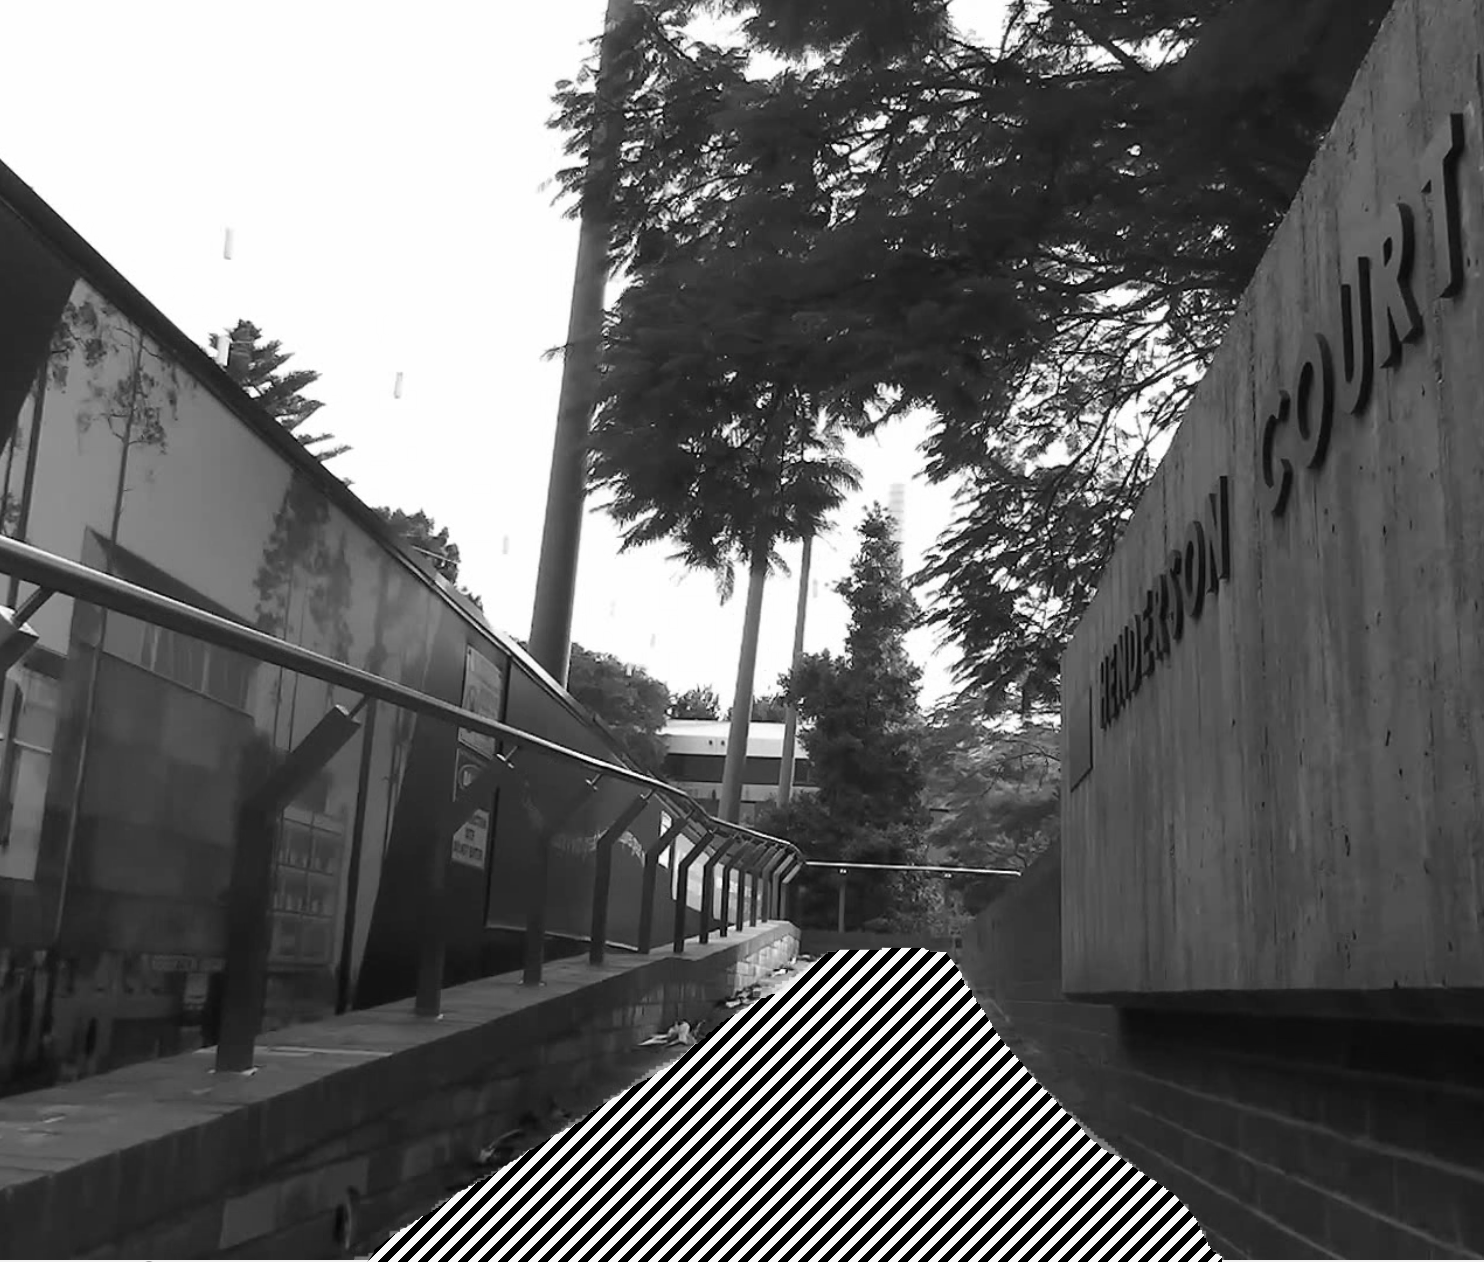
\includegraphics[width=\linewidth]{images/segmentation_gs.png}
    \end{subfigure}
    \quad
    \begin{subfigure}{.2\textwidth}
        \centering
        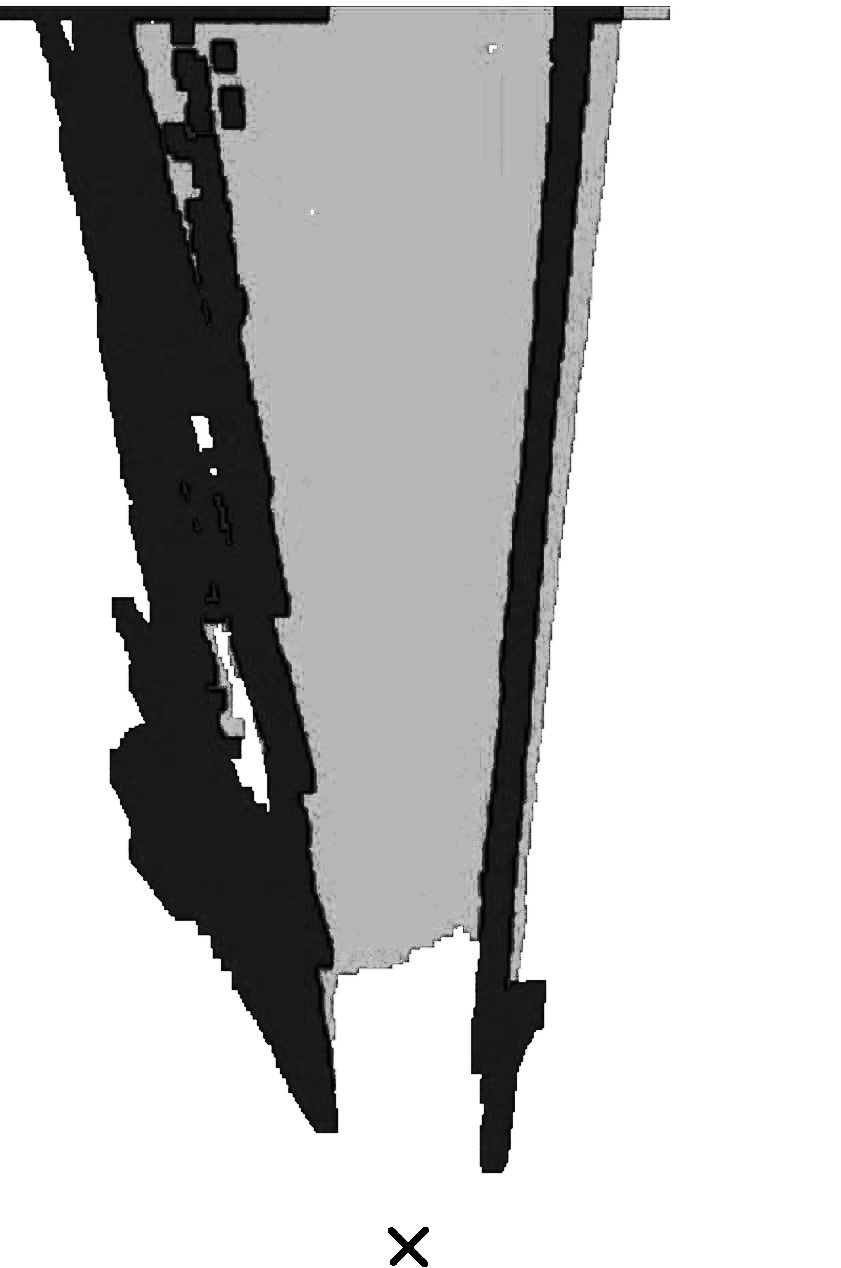
\includegraphics[width=\linewidth,frame]{images/map_gs.png}
    \end{subfigure}
    \caption{Drivable area segmentation and obstacle detection (top-down occupancy map)}
    \label{fig:algorithm}
\end{figure}

%\begin{minipage}[c]{\textwidth}
%    \centering
%    \includegraphics[width=3.0in]{example-image-a}
%    \captionof{figure}{Caption for image}
%    \label{fig:sample_figure}
%^\end{minipage}

\section*{\textbf{CONCLUSIONS}} % 5 lines
The results indicate that image segmentation is effective at identifying drivable areas outdoors.
The custom 3D point cloud processing algorithm works well at identifying walls,
however, is not yet fast enough for moving objects such as pedestrians.
The navigation assistance technology developed and tested in this thesis can be integrated
with other thesis students' work to create a semi-autonomous wheelchair. To work around the FOV
of the RGB-D camera, a SLAM algorithm could be used to keep obstacles in memory.

%\section*{\textbf{ACKNOWLEDGEMENTS}}
%The author wishes to thank Glide for providing a powered wheelchair to the research team.

\printbibliography[title=\textbf{REFERENCES},heading=bibliography] % don't need titles for journal articles, just page #

\end{document}
